
% Brechungsindex theorie $n = 3,73$


\nocite{anleitungV407}
\section{Auswertung}
\label{sec:Auswertung}
Die zu Erst gemessenen Werte des Nullstroms $I_0$ und des Dunkelstroms $I_{\text{D}}$ lauten
\begin{align*}
  I_0 &= 460\,\unit{\micro\ampere}\\
  I_{\text{D}} &= 2,8\,\unit{\nano\ampere}\,.
\end{align*}
Wärhend der Messung des Dunkelstroms, ist das Photoelement einer maximalen Störung von anderen Lichtquellen ausgesetzt. Bei der Durchführung treffen nur minimale Störungen auf
das Photoelement. Zusätzlich befindet sich die maximale Störung in einem kleinen Bereich, weswegen der Dunkelstrom im weiteren Verlauf der Auswertung vernachlässigt wird.

\subsection{Berechnung des Brechungsindex}
\begin{table}[H]
  \centering
  \caption{Gemessene Photoströme bei s- und p-polarisiertem Licht in Abhängigkeit vom Einfallswinkel $\alpha$.}
  \label{tab:Messwerte}
  \begin{tblr}{colspec={c c c|| c c c|| c c c}}
      \toprule
      $\alpha\,[°]$ & $I_{\text{ref, s}}\,[\unit{\micro\ampere}]$ & $I_{\text{ref, p}}\,[\unit{\micro\ampere}]$ & $\alpha\,[°]$ & $I_{\text{ref, s}}\,[\unit{\micro\ampere}]$ & $I_{\text{ref, p}}\,[\unit{\micro\ampere}]$ & $\alpha\,[°]$ & $I_{\text{ref, s}}\,[\unit{\micro\ampere}]$ & $I_{\text{ref, p}}\,[\unit{\micro\ampere}]$ \\
      \midrule  
      6   &   6   &   14  &   38  &   24  &   20  &   70  &   110 &   3   \\
      8   &   8   &   14  &   40  &   31  &   20  &   71  &   120 &   1   \\
      10  &   7   &   15  &   42  &   28  &   20  &   72  &   120 &   2,2 \\
      12  &   10  &   15  &   44  &   39  &   20  &   73  &   130 &   1,4 \\
      14  &   6   &   14  &   46  &   38  &   20  &   74  &   140 &   0,9 \\
      16  &   11  &   11  &   48  &   47  &   20  &   75  &   140 &   0,5 \\
      18  &   10  &   16  &   50  &   46  &   20  &   76  &   130 &   0,57\\
      20  &   10  &   16  &   52  &   55  &   19  &   77  &   150 &   0,76\\
      22  &   12  &   16  &   54  &   64  &   17  &   78  &   140 &   1,5 \\
      24  &   15  &   17  &   56  &   70  &   16  &   79  &   160 &   2,8 \\
      26  &   12  &   17  &   58  &   70  &   16  &   80  &   150 &   4,6 \\
      28  &   17  &   18  &   60  &   80  &   14  &   82  &   170 &   10  \\
      30  &   14  &   18  &   62  &   78  &   12  &   84  &   160 &   23  \\
      32  &   19  &   19  &   64  &   90  &   10  &   86  &   190 &   43  \\
      34  &   18  &   19  &   66  &   90  &   8   &   87  &   190 &   60  \\
      36  &   26  &   19  &   68  &   110 &   5   &   &   & \\      
      \bottomrule
  \end{tblr}
\end{table}
In der Tabelle \ref{tab:Messwerte} sind die gemessenen Photoströme in Abhängigkeit des Einfallswinkels $\alpha$ aufgelistet.
Um die Brechungsindizes für s- und p-polarisiteres Licht zu bestimmen, werden die Gleichungen (\ref{eqn:}) und (\ref{eqn:}) nach $n_{\text{s}}$ und $n_{\text{p}}$
umgestellt. Daraus ergeben sich
\begin{align}
  n_{\text{s}} &= \sqrt{\frac{E^2 - 2E\cos(2\alpha) + 1}{E^2- 2E + 1}} \label{eqn:n_s} \qquad {\text{und}}\\
  n_{\text{p}} &= \sqrt{\left(\frac{1+E}{1-E}\right)^2 \frac{1}{2\cos^2(\alpha)} + \sqrt{\frac{(1+E)^2}{4\cos^4(\alpha)(1-E)^4}- \frac{1}{(1-E)^2} \tan^2(\alpha)}} \label{eqn:n_p}\,.
  % n_{\text{p}} &= \sqrt{\frac{(1+E)^2}{(1-E)^2}\frac{1}{2\cos^2(\alpha)} + \frac{\sqrt{(1+E)^2-4\cos^2(\alpha)(1-E)^2\sin^2(\alpha)}}{2\cos^2(\alpha)(1-E)^2}}
\end{align}
Hierfür gilt $$E = \frac{E_{\text{ref}}}{E_{\text{ein}}} = \frac{I_{\text{ref}}(\alpha)}{I_0}\,.$$
Die berchneten Brechungsindizes sind in der Tabelle \ref{tab:Brechungsindex} aufgeführt. Durch systematische Fehler werden allerdings für das s-polarisierte Licht
die Werte $n_{\text{s}} > 4$ und bei dem p-polarisiertem Licht alle Werte $n_{\text{p}} > 6$ vernachlässigt. Die daraus gemittelten Brechungsindizes sind
\begin{align*}
  \overline{n_{\text{s}}} &= 2,0\pm 0,9\quad \text{und}\\
  \overline{n_{\text{p}}} &= 2,4\pm 1,1\,.
\end{align*}
Die Messdaten sind in der Abbildung \ref{fig:plot} dargestellt. Hierbei ist $\sqrt{\sfrac{I(\alpha)}{I_0}}$ gegen $\alpha$ aufgetragen. Zusätzlich sind in der Abbildung
die Theoriekurven abgebildet, welche durch $\overline{n_{\text{s}}}$, $\overline{n_{\text{p}}}$ sowie den Gleichungen (\ref{eqn:}) und (\ref{eqn:}) bestimmt werden.
\begin{figure}
  \centering
  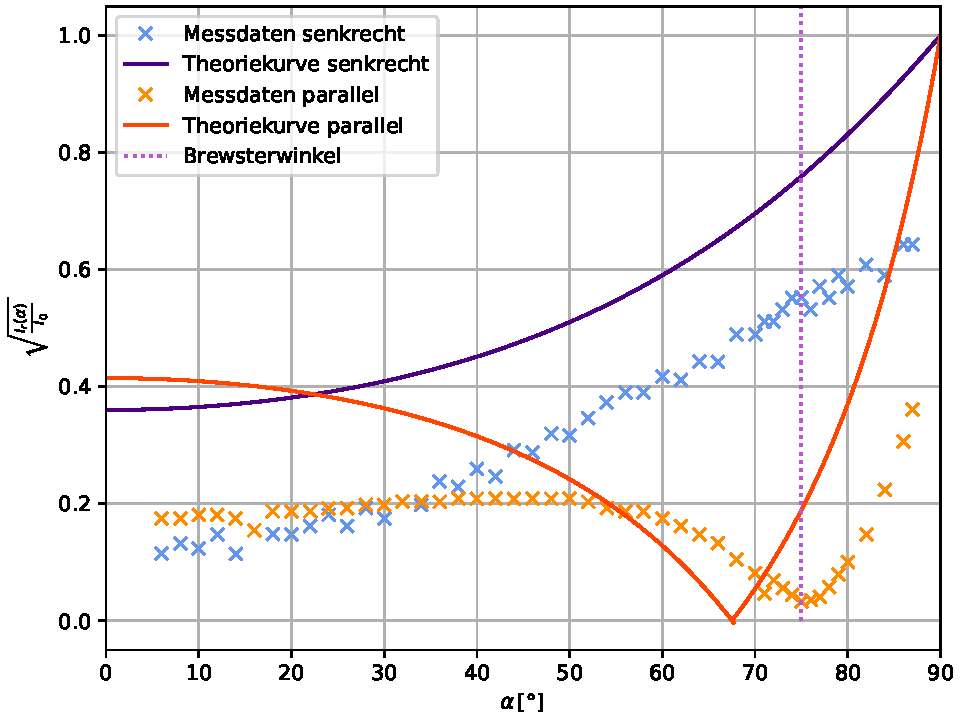
\includegraphics[width=0.8\textwidth]{plot.pdf}
  \caption{Graphische Darstellung der Messwerte mit der Theoriekurve und markiertem Brewsterwinkel.}
  \label{fig:plot}
\end{figure}
Außerdem wird anhand der Tabelle beim Minimum des p-polarisitem Licht ein Brewsterwinkel von $\alpha_{\text{B}} = 75\,°$ abgelesen. Dieser ist ebenfalls in der Abbildung \ref{fig:plot} eingezeichnet.
Anhand dieses Brewsterwinkels lässt sich über die Gleichung (\ref{eqn:}) der theoretische Brechungsindex $$n = 3,73$$ ermitteln.
  \begin{table}[H]
    \centering
    \caption{Brechnete Brechungsindizes in Abhängigkeit des Winkels und der Intensität.}
    \label{tab:Brechungsindex}
    \begin{tblr}{colspec={c c c|| c c c|| c c c}}
        \toprule
        $\alpha\,[°]$ & $n_{\text{s}}$ & $n_{\text{p}}$ & $\alpha\,[°]$ & $n_{\text{s}}$ & $n_{\text{p}}$ & $\alpha\,[°]$ & $n_{\text{s}}$ & $n_{\text{p}}$ \\
        \midrule  
        6   &   1,00  &   1,37  & 38&   1,26  &   1,75  &   70  &   2,76 &   3,24\\
        8   &   1,01  &   1,38  & 40&   1,34  &   1,80  &   71  &   2,94 &   3,19\\
        10  &   1,01  &   1,40  & 42&   1,33  &   1,85  &   72  &   2,95 &   3,53\\
        12  &   1,02  &   1,40  & 44&   1,46  &   1,91  &   73  &   3,14 &   3,64\\
        14  &   1,02  &   1,39  & 46&   1,47  &   1,98  &   74  &   3,34 &   3,80\\
        16  &   1,03  &   1,35  & 48&   1,59  &   2,06  &   75  &   3,35 &   3,98\\
        18  &   1,04  &   1,44  & 50&   1,61  &   2,15  &   76  &   3,18 &   4,29\\
        20  &   1,05  &   1,45  & 52&   1,73  &   2,22  &   77  &   3,58 &   4,67\\
        22  &   1,06  &   1,47  & 54&   1,87  &   2,27  &   78  &   3,39 &   5,23\\
        24  &   1,09  &   1,50  & 56&   1,97  &   2,37  &   79  &   3,81 &   5,94\\
        26  &   1,08  &   1,52  & 58&   2,00  &   2,51  &   80  &   3,61 &   6,81\\
        28  &   1,12  &   1,56  & 60&   2,16  &   2,60  &   82  &   4,06 &   9,31\\
        30  &   1,12  &   1,58  & 62&   2,17  &   2,71  &   84  &   3,86 &   14,34\\
        32  &   1,17  &   1,63  & 64&   2,37  &   2,84  &   86  &   4,59 &   25,32\\
        34  &   1,18  &   1,66  & 66&   2,40  &   2,98  &   87  &   4,59 &   37,91\\
        36  &   1,25  &   1,69  & 68&   2,73  &   3,08  &   &   & \\      
        \bottomrule
    \end{tblr}
  \end{table}


